\documentclass{BYUTextbook}

\usepackage[dutch]{babel}

\usepackage{parskip}
\usepackage{graphicx}
\usepackage{hyperref}
\usepackage{needspace}
\sloppy
%%% ---------------  onze definities ----------------

% app inventor kleuren
\definecolor{aiblue}{rgb}{0.65,.78,0.9}
\definecolor{aigreen}{rgb}{0.81,.87,0.6}

% \ai voor 'App Inventor' (ik word zo moe van steeds die hoofdletters in te moeten typen :-) )
\newcommand{\ai}[0]{\emph{App Inventor} \nolinebreak}

% gebruik \block voor een block in de AppInventor-block editor   ( voor nu: italic bold )
\newcommand{\block}[1]{\colorbox{aiblue}{ \texttt{#1} }}

\newcommand{\menuitem}[1]{\colorbox{aigreen}{ #1 }} 

\newcommand{\bestand}[1]{\url{#1}}  % eigenlijk is het gebruik van url hier niet helemaal correct omdat de link nergens naartoe wijst, maar het ziet er wel OK uit. 

% Run op telefoon
\newcommand{\runOpTelefoon}[2][0pt]{
    \marginpar{\captionsetup{type=table} \vspace{#1}
    \begin{minipage}[t][#2]{1.23in}
    \smallskip
    \footnotesize 
    \checkoddpage
    \ifoddpage
	   \RaggedRight 
    \else
	   \RaggedLeft
    \fi
    
\includegraphics[width=.615in]{screenshots/run_op_telefoon}
	    
    \end{minipage}
    }
}


% Metadata, licentie
\ifpdf
\pdfinfo {
/Title (Android Apps met App Inventor - Docentenhandleiding)
/Author (Coen Crombach, Robin Eggenkamp, Fran\c{c}ois Vonk � CC-Licence : http://creativecommons.org/licenses/by-nc-sa/3.0/)
}
\fi

\includexmp{creativecommons}

%%% ---------------  begin van het document ----------------
\begin{document}

\frontmatter

\thispagestyle{empty}
\begin{adjustwidth}{}{-1.5in}

 \centering
 \vspace{.6in}
 \Huge Android Apps met App Inventor
 
 \Huge Docentenhandleiding
 \normalsize
 \vspace{.6in}

Coen Crombach

Robin Eggenkamp

Fran\c{c}ois Vonk

 \vspace{0.4in}

% \graphicspath{{screenshots/building_blocks/}{screenshots/AppInventorLogo/}}
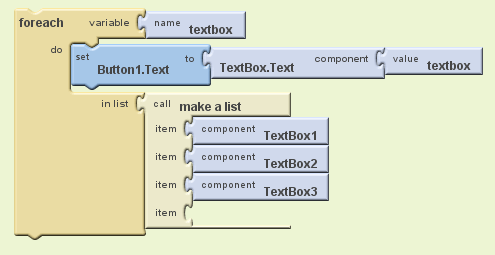
\includegraphics[width=\textwidth]{screenshots/building_blocks}

\vspace{0.25in}


\includegraphics[width=0.5\textwidth]{screenshots/AppInventorLogo}

 \vspace{.6in}

\today


\end{adjustwidth}

\null
\vfill
\ccbyncsaeu

\small{Dit werk is gelicenseerd onder een Creative Commons Naamsvermelding-NietCommercieel-GelijkDelen 3.0 Unported. Bezoek \url{http://creativecommons.org/licenses/by-nc-sa/3.0/} om een kopie te zien van de licentie of stuur een brief naar Creative Commons, 444 Castro Street, Suite 900, Mountain View, California, 94041, USA.}

\cleardoublepage

\tableofcontents

\mainmatter

\chapter{Inleiding}
\begin{derivation}{Noot}
  Het lesmateriaal dat u hebt gekregen is nog niet af! Zaken zoals lay-out en schrijfstijl zijn bijvoorbeeld nog niet altijd consistent. Ook is het materiaal nog niet helemaal compleet. Het materiaal is volgens ons echter van voldoende kwaliteit om er een oordeel over te vormen en aan te geven of het zinvol is om het af te maken of dat we mogelijk zaken anders aan moeten pakken. Hierover willen we dan ook graag feedback. We zijn in het bijzonder ge\"interesseerd in uw mening over motiverende werking en effectiviteit.
\end{derivation}

Beste docent. Dit is de docenten handleiding bij het lesmateriaal Android Apps met \ai. Het lesmateriaal is zo opgezet dat leerlingen die dit willen zelfstandig kunnen werken. In het lesmateriaal zijn opgaven verwerkt die makkelijk herkend kunnen worden door de manier waarop we ze vorm hebben gegeven, zie figuur \ref{screenshots/docent_opgave}. Hierdoor kunnen meerdere lesstrategie\"en tegelijkertijd worden toegepast:

\begin{itemize}
  \item Leerlingen kunnen zelfstandig de opdrachten in het materiaal zoeken en proberen die te maken door eerst zelf zo ver mogelijk te komen en op te zoeken wat ze niet weten.
  \item Leerlingen kunnen zelfstandig gaan lezen en opdrachten maken wanneer ze die tegenkomen.
  \item Leerlingen kunnen zelfstandig eerst alles doorlezen en daarna opdrachten gaan maken.
  \item Je kunt als docent de hele klas of die leerlingen uit de klas die daar behoefte aan hebben een aantal stappen uit het materiaal voordoen en de leerlingen het dan na laten doen.
\end{itemize}

Dit biedt de mogelijkheid om leerlingen met verschillende leerstijlen op een voor hen fijne manier aan het werk te zetten en ze daardoor beter te bedienen. \\
In hoofdstukken 1 (Installatie) en 2 (Ontwikkelomgeving) staan nog geen opgaven. Het is daarom raadzaam alle leerlingen die twee hoofdstukken eerst door te laten lezen.

\inlinefig{screenshots/docent_opgave}{Opmaak van een opgave in het materiaal}

We raden aan om als docent een Google account te hebben zodat je zelf de \ai ontwikkelomgeving kunt gebruiken. Hieronder de relevante links (die natuurlijk ook in het lesmateriaal staan):
\begin{itemize}
  \item \url{accounts.google.com/NewAccount?hl=nl}
  \item \url{beta.appinventor.mit.edu}
\end{itemize}
Ook raden we aan om toegang tot een dummy leerling schoolaccount te hebben zodat je kunt testen of alles werkt voor de leerlingen. Dit voorkomt vervelende verrassingen tijdens de eerste les.

\chapter{Opzet van het materiaal}
Na de uitleg van de installatie en ontwikkelomgeving beginnen we met een luchtig spel genaamd Mollen Meppen. We laten de leerlingen hier allereerst kennismaken met de emulator. We raden aan de leerlingen niet te vroeg naar een echt Android apparaat te laten gaan omdat we het gebruik van de emulator ook belangrijk vinden. Bovendien wil je in het begin dat leerlingen met de ontwikkelomgeving bezig zijn en niet met hun mobieltje. Als ze alle opgaven van Mollen Meppen hebben gemaakt (behalve de bonus opgave) is het een mooi moment om het op hun telefoon te testen.

In het lesmateriaal worden elementen uit de ontwikkelomgeving met een aparte opmaak weergegeven. Voor items uit de menu's gebruiken we tekst op een licht groene achtergrond en voor programmeerblokken (blocks) gebruiken we tekst op een licht blauwe achtergrond. Dit staat uiteraard ook uitgelegd in het lesmateriaal zelf.

Bij het lesmateriaal worden ook projecten bijgeleverd die als startpunt voor de leerlingen dienen. Omdat scholen verschillende leeromgevingen hebben kunnen we in ons lesmateriaal geen informatie verschaffen over waar deze projecten te vinden zijn. Het handigst is het als de leerlingen dit al weten voor ze met het materiaal aan de slag gaan. Op punten waar zij iets nodig hebben geven we in het lesmateriaal aan dat ze bij de docent kunnen informeren waar het \'e\'en en ander staat.

Het lesmateriaal begint vrij eenvoudig en wordt gaandeweg moeilijker. We zetten eerst de basis in de steigers (scaffolding) en bouwen daar vervolgens op verder. Ook worden belangrijke concepten herhaald om ze goed te verankeren. Ieder hoofdstuk heeft verder \'e\'en of meerdere bonus opgaven zodat leerlingen die snel door het lesmateriaal gaan extra uitdagingen krijgen.

In figuur \ref{screenshots/docent_opbouw} staat een schema dat aangeeft welke \ai- en programmeerconcepten aan bod komen in de diverse onderdelen van het lesmateriaal. De verschillende fontkleuren in het figuur geven de volgorde in het lesmateriaal aan. Concepten in rode tekst behoren bij Mollen Meppen, groene tekst bij Schrandere Scholier en blauwe tekst bij Meteoor. De doorgetrokken pijlen geven afhankelijkheidsrelaties aan. Zo hebben we ervoor gekozen een leerling eerst code te laten lezen voordat hij/zij met het design scherm aan de slag gaat. Voordat een leerling echter zelf gaat programmeren moet deze eerst een beperkte kennis van het design scherm hebben. De onderbroken pijlen geven herhaling weer en staan alleen tussen concepten met gelijke namen. Concepten die op dezelfde hoogte staan in het figuur hebben geen relatie of afhankelijkheid ten opzichte van elkaar.

Een aantal concepten in figuur \ref{screenshots/docent_opbouw} verdienen enige toelichting:
\begin{itemize}
  \item Met design scherm bedoelen we gebruik van menu's en componenten.
  \item Met selectie bedoelen we het conditioneel uitvoeren van stukken code met bijvoorbeeld een if-statement.
  \item Met events bedoelen we gebeurtenissen gegenereerd door standaard componenten, zoals het indrukken van een knop.
  \item Met sprites worden bewegende objecten bedoeld.
  \item We hebben botsen detecteren gebruikt als vertaling van Collision Detection.
\end{itemize}
 
\inlinefig{screenshots/docent_opbouw}{Scaffolding en herhaling}

In het lesmateriaal is niet specifiek rekening gehouden met vrouwelijke leerlingen of allochtone leerlingen. De onderwerpen zijn naar onze mening redelijk neutraal van aard op het gebied van deze vormen van diversiteit.

Op het moment schatten we de benodigde tijd per onderwerp als volgt in:
\begin{itemize}
  \item Introductie en Mollen Meppen 4 lesuren
  \item Schrandere Scholier 6 lesuren
  \item Meteoor 6 lesuren
  \item Onderwerp waarin we procedures met parameters gebruiken en liefst variabelen, selectie en loops herhalen 6 lesuren \emph{(nog te ontwikkelen)}
  \item Vrije individuele opdracht 10 uren \emph{(nog te ontwikkelen)}
  \item Vrije groepsopdracht 15 uren \emph{(nog te ontwikkelen)}
\end{itemize}

Dit is in totaal 47 uur wat uitkomt op bijna 16 weken bij 3 uur les per week. Vrij vertaald zou dit moeten passen in 2 perioden van ongeveer 8 weken.

\chapter{Achtergrond bij keuzes gemaakt in het materiaal}
Ons doel met het lesmateriaal was het maken van een lessenserie die leerlingen motiveert om te leren programmeren en die dit vervolgens op een effectieve manier doet.

Het gekozen platform is ons grootste motiverende aspect. Echter het niet hoeven omgaan met vaak lastig te interpreten compiler of interpreter meldingen omdat we voor een grafische ontwikkelomgeving hebben gekozen zal voorkomen dat leerlingen gedemotiveerd raken.

Voor startende programmeurs is een grafische ontwikkelomgeving een effectieve manier voor het leren van programmeerconcepten om de volgende redenen:
\begin{itemize}
  \item Syntax van tekstuele programmeertalen leidt af van de programmeerconcepten.
  \item Lastig te interpreteren meldingen van compilers en interpreters kosten vaak veel tijd die niet besteed kan worden aan het leren programmeren.
  \item Grafische bouwblokken die in elkaar klikken geven direct feedback over de semantiek van de bouwblokken zodat leerlingen niet steeds hoeven te zoeken naar de regels zoals bij tekstuele programmeertalen.
\end{itemize}

Onder programmeerconcepten verstaan we dingen als variabelen, selectief code uitvoeren, herhaald code uitvoeren (loops), events, testen, debuggen enzovoorts. Als leerlingen eenmaal bekend zijn met de programmeerconcepten kunnen ze veel makkelijker en sneller overstappen naar een tekstuele ontwikkelomgeving omdat ze ook moeten ervaren hoe deze werken. Met name testen en debuggen is heel anders in dit type omgevingen.

Zeker in het begin bij Mollen Meppen hebben we ervoor gekozen om de leerling steeds iets kleins te laten wijzigen zodat er voldoende succesmomenten zijn. Dit zal bijdragen aan de motivatie van leerlingen om door te gaan.

Als eerste ervaring met programmeren hebben we er voor gekozen om de leerlingen al iets te geven dat werkt maar nog verre van perfect is. Dit is een goed beginpunt om voor het eerst een app uit te voeren in de ontwikkelomgeving. De opzet is dusdanig eenvoudig dat leerlingen het moeten kunnen begrijpen. Daarna mogen de leerlingen zelf dingen in de code veranderen en er dingen bij maken. Dit sluit aan bij de "cognitieve doelen strategie" van Jens Kaasb\o ll (Kaasb\o ll, 1998). In deze strategie onderkent Kaasb\o ll 4 stappen:
\begin{enumerate}
  \item Voer een programma uit
  \item Lees de code van een programma
  \item Breng veranderingen aan in een programma
  \item Schrijf zelf een programma
\end{enumerate}

Onderdeel van deze strategie is tevens het "programmeren door completeren" zoals beschreven door Merri\"{e}nboer (Merri\"{e}nboer, 1992). Dit wordt doorgaans ook als een goede didactische aanpak gezien bij het beginnen met leren programmeren.

Verder hebben we gepoogd zoveel mogelijk van de zogenaamde Big Ideas van programmeren (Saeli, 2012) aan bod te laten komen omdat Informatica docenten deze belangrijk vinden binnen het programmeeronderwijs:
\begin{itemize}
  \item Controle structuren met de focus op loops
    \begin{itemize}
      \item In Schrandere Scholier bij het doorlopen van een lijst
    \end{itemize}
  \item Data structuren
    \begin{itemize}
      \item De ontwikkelomgeving kent getallen, booleans en tekst als data structuren maar dit is een zeer klein begin en booleans zijn zeer impliciet
      \item In Schrandere Scholier wordt de datastructuur lijst gebruikt
    \end{itemize}
  \item Arrays
    \begin{itemize}
      \item Zitten niet in de ontwikkelomgeving en komen daarom niet als zodanig aan bod
      \item In Schrandere Scholier worden wel lijsten gebruikt die feitelijk een meer algemene vorm van een array zijn
    \end{itemize}
  \item Probleem oplossende vaardigheden
    \begin{itemize}
      \item Worden aangesproken in de opgaven in het lesmateriaal
    \end{itemize}
  \item Decompositie
    \begin{itemize}
      \item In lichte mate in Mollen Meppen door met een procedure te werken in de versie die de leerlingen krijgen maar er wordt hier niet direct op gestuurd
      \item In Schrandere Scholier moeten leerlingen zelf een procedure maken
    \end{itemize}
  \item Parameters
    \begin{itemize}
      \item In Schrandere Scholier worden deze genoemd maar de leerlingen hoeven er nog niet mee aan de slag
    \end{itemize}
  \item Algoritmes
    \begin{itemize}
      \item In lichte mate in Mollen Meppen door het laten tellen van missers en het inbouwen van een score
      \item In lichte mate in Schrandere Scholier door het laten berekenen welk cijfer er gehaald moet worden voor een 8 gemiddeld
      \item In Meteoor bij het werken met de hellingshoek van het mobiele apparaat
    \end{itemize}
\end{itemize}
    
\chapter{Tot slot}
Het materiaal zoals het er nu ligt is wat ons betreft nog niet af. Er staan nog een aantal onderwerpen in de rij. Na het doorlopen van de onderwerpen raden we aan om leerlingen eerst individueel een App te laten bedenken en maken. Hiermee kun je toetsen of alle leerlingen iets hebben opgestoken van de programmeerconcepten. Vervolgens is het misschien leuk om leerlingen in groepjes een wat grotere App te laten bedenken en maken. Hierbij is het wellicht leuk om leerlingen educatieve Apps te laten maken die aansluiten bij \'e\'en van de andere vakken die ze hebben zoals biologie, geschiedenis, aardrijkskunde enzovoorts.

\chapter{Referenties}
Kaasb\o ll, J.J. (1998). Exploring didactic models for programming. Tapir, pp. 195-203.

Merri\"{e}nboer, J.J.G. van (1992). Programmeren door completeren. TINFON, 1(2), pp. 66-71.

Saeli, M. (2012, February). Teaching Programming for Secondary School: a Pedagogical Content Knowledge Based Approach. Technische Universiteit Eindhoven.

\cleardoublepage

\end{document}